Sacramento Municipal Utility District (SMUD), which is the nation's sixth-largest community-owned electric utility, provides electricity to most of Sacramento County and small portions of adjoining Placer and Yolo Counties.\footnote{According to the company information presented on \href{https://www.smud.org/en/Corporate/About-us/Company-Information}{SMUD's website}, the size of this utility's service area is about 900 square miles.}

\afterpage{
    \begin{figure}[t!]
        \centering
        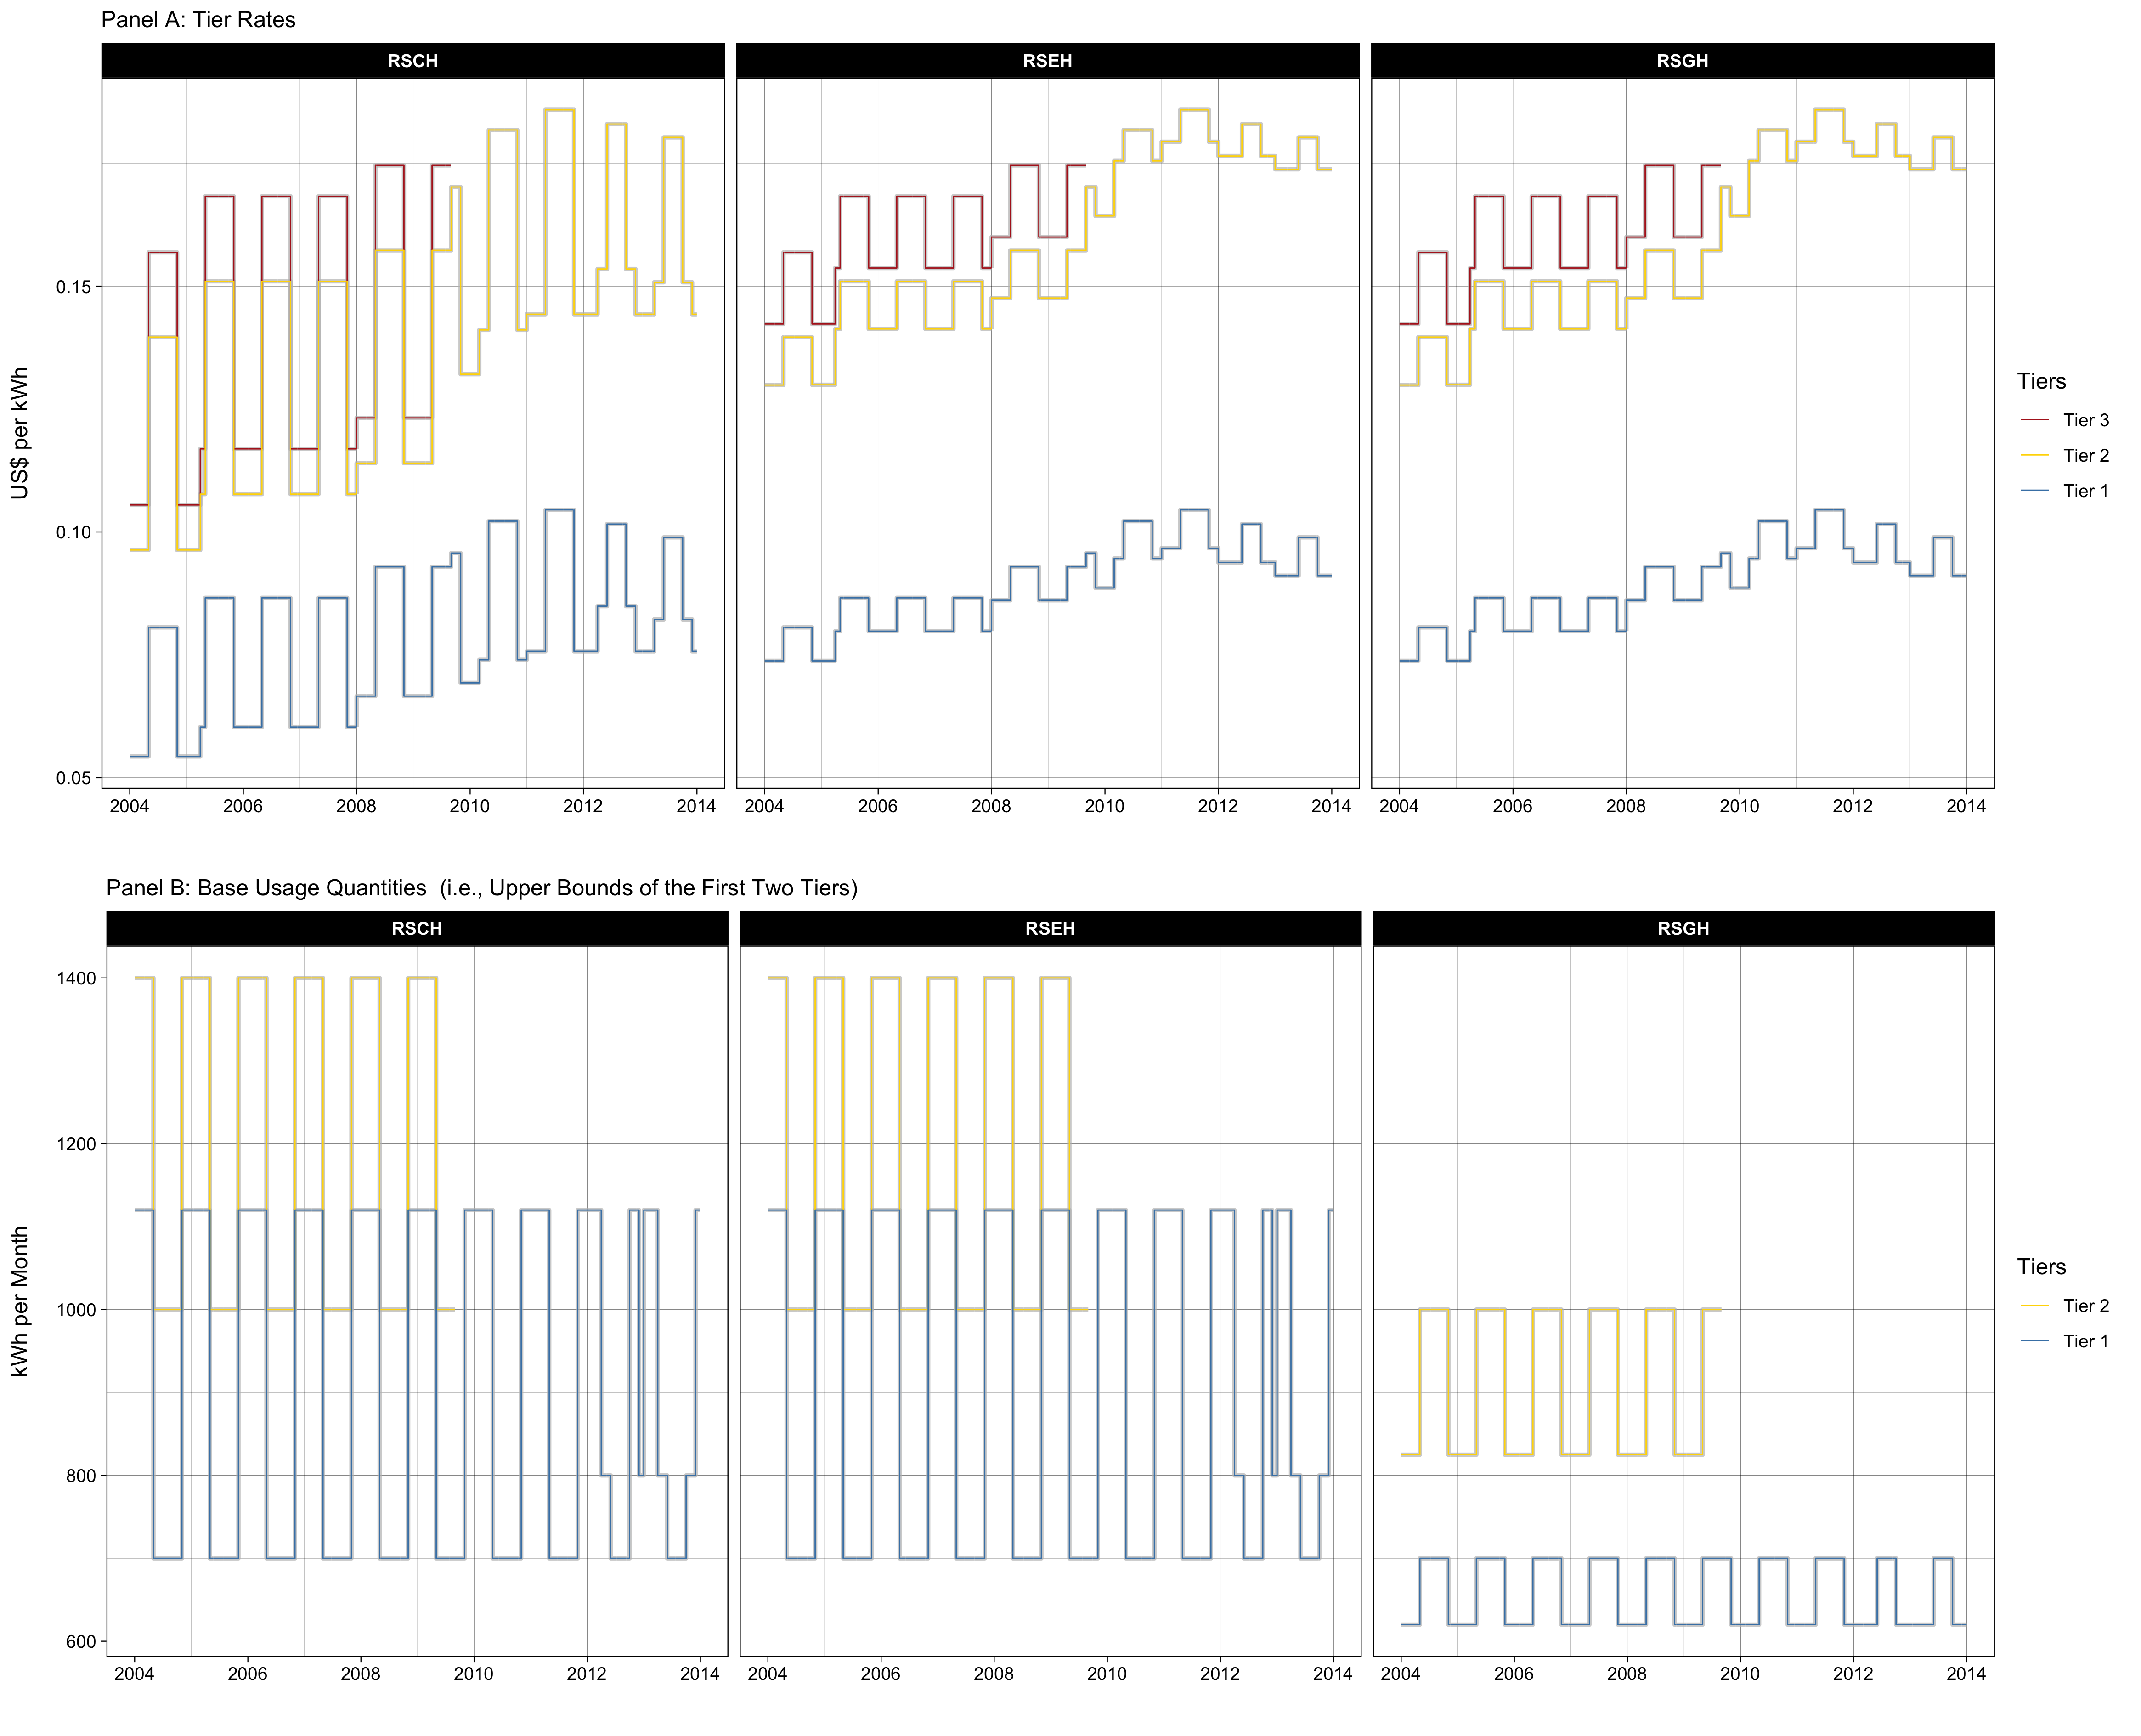
\includegraphics[scale = 0.097]{02_Chapter-1/00A_Figures/Figure_SMUD-Residential-Rates_Variable-Charges-and-Base-Usage-Quantities.png}
        \caption{Tier Rates and Base Usage Quantities of SMUD Residential Rates}
        \caption*{
            {\small
            \textit{Note}: 
            The figure illustrates how SMUD changed tier rates and base usage quantities of the three major residential rate plans (i.e., RSCH, RSEH, and RSGH) over time. Both tier rates and base usage quantities show significant seasonality. The two rate plans for electric-heating households (i.e., RSCH and RSEH) had the same base usage quantities. There have been only two tiers since September 2009.
        }}
        \label{Figure:SMUD-Residential-Rates_Variable-Charge-and-Base-Usage}
    \end{figure}
}
Before the default residential rate switched to the Time-Of-Day (TOD) rate, most SMUD residential customers chose residential rates having an increasing nonlinear block-tier structure.\footnote{In my sample, only 5\% of residential customers adopted the TOD rate, although SMUD already offered it.} The three most popular rates for SMUD residential customers were Standard General Service (RSGH), Standard Closed Electric-Heated Service (RSCH), and Standard Open Electric-Heated Service (RSEH).\footnote{Specifically, more than 75\% of SMUD residential customers in my dataset chose the RSGH rate, whereas 2\% and 20\% of households in my dataset adopted the RSCH and RSEH rates, respectively.} For those residential rates, the marginal price of the energy charge was a step function of monthly consumption relative to a base usage quantity per month, which varies seasonally. Figure \ref{Figure:SMUD-Residential-Rates_Variable-Charge-and-Base-Usage} illustrates variations in price and base usage quantity over time. Two points are noteworthy from this figure: first, both tier rates and base usage quantities of the energy charges showed substantial seasonality; second, the structure of the residential rates changed from three-tier to two-tier since September 2009.

In addition to the variable charge (i.e., the energy charge), households choosing one of the three rates should pay a per-month fixed charge, called the System Infrastructure Fixed Charge. As shown in Figure \ref{Figure:SMUD-Residential-Rates_Fixed-Charge}, the unit price of the fixed charge significantly increased between 2009 and 2014. 
